\section{Approach Overview}
\label{sec:approach}


\begin{figure}[t]
\centering
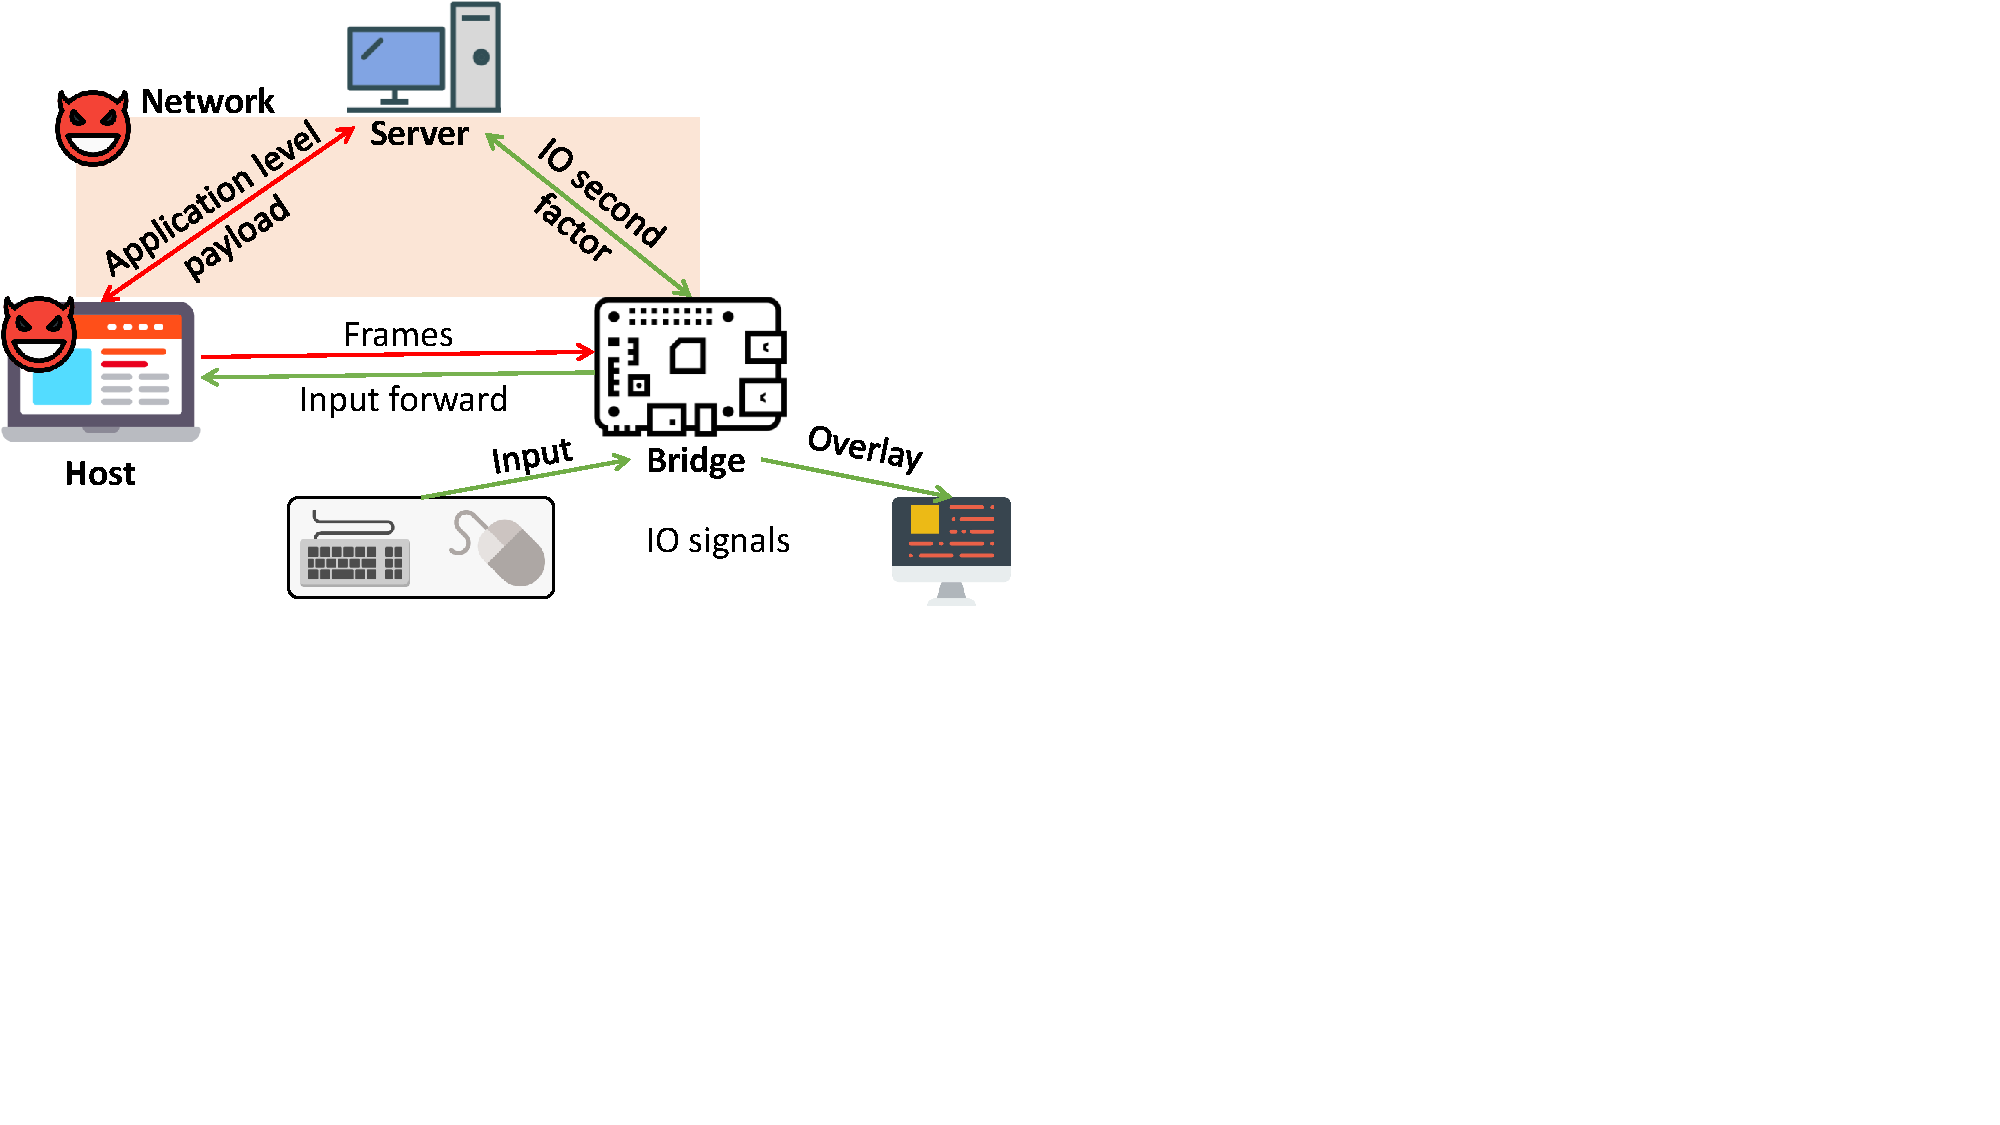
\includegraphics[trim={0 6cm 17cm 0}, clip, width=0.85\linewidth]{approachOverview.pdf}
\caption{\textbf{High-level approach overview of our solution.}  The \device connects the IO devices and the attacker-controlled host. }
\label{fig:approachOverview}
\centering
\end{figure}


In this section, we describe an overview of our proposed solution. As described in the problem statement discussed in Section~\ref{sec:problemStatement}, our proposed solution provides a trusted path between the user IO device and the remote server by utilizing a trusted embedded device as a mediator between all the IO devices and the untrusted host. We call this device: \device. The approach, on the high-level, uses the concept of the \emph{bump in the wire}~\cite{McCPerRei2006} to provide integrity and privacy to the user IO actions. The overall approach is illustrated in Figure~\ref{fig:approachOverview}. On a high level, the remote server and the \device establishes a secure channel using the untrusted host as a transport. Note that the \device does not have any network capabilities, instead uses the host as an untrusted transport. The server also adds a small JavaScript snippet that allows the \device and the remote server to communicate. This eliminates any need for additional hardware/software aids.

We first define the system and attacker model, then outline the challenges and the brief outline of our proposed solution.

%Given the problem statement discussed in Section~\ref{sec:problemStatement}, we first define the attacker model we consider in our proposed system.


\subsection{System and Attacker Model}

We consider a system model where the user wants to sends the input to a safety-critical remote end-system. The model is depicted in Figure~\ref{fig:approachOverview} that shows the compromised host, remote server and the user IO devices. 

We assume that the attacker compromises the host system completely (OS, installed applications and hardware). The attacker also controls the network. We only assume that it is a PPT-attacker, so he can not break crypto. Figure~\ref{fig:systemModel} shows the components of the system that are controlled by the attacker, i.e., the host and the network communication channel between the host and the remote server.

We only assume that the monitor, keyboard, mouse (in a word all the IO devices that we need to protect from the malicious host) and the \device are trusted, which is not unrealistic. The monitor, keyboard, and mouse have hardly any complex hardware. The TCB is very small.

\iffalse
\begin{figure}[t]
\centering
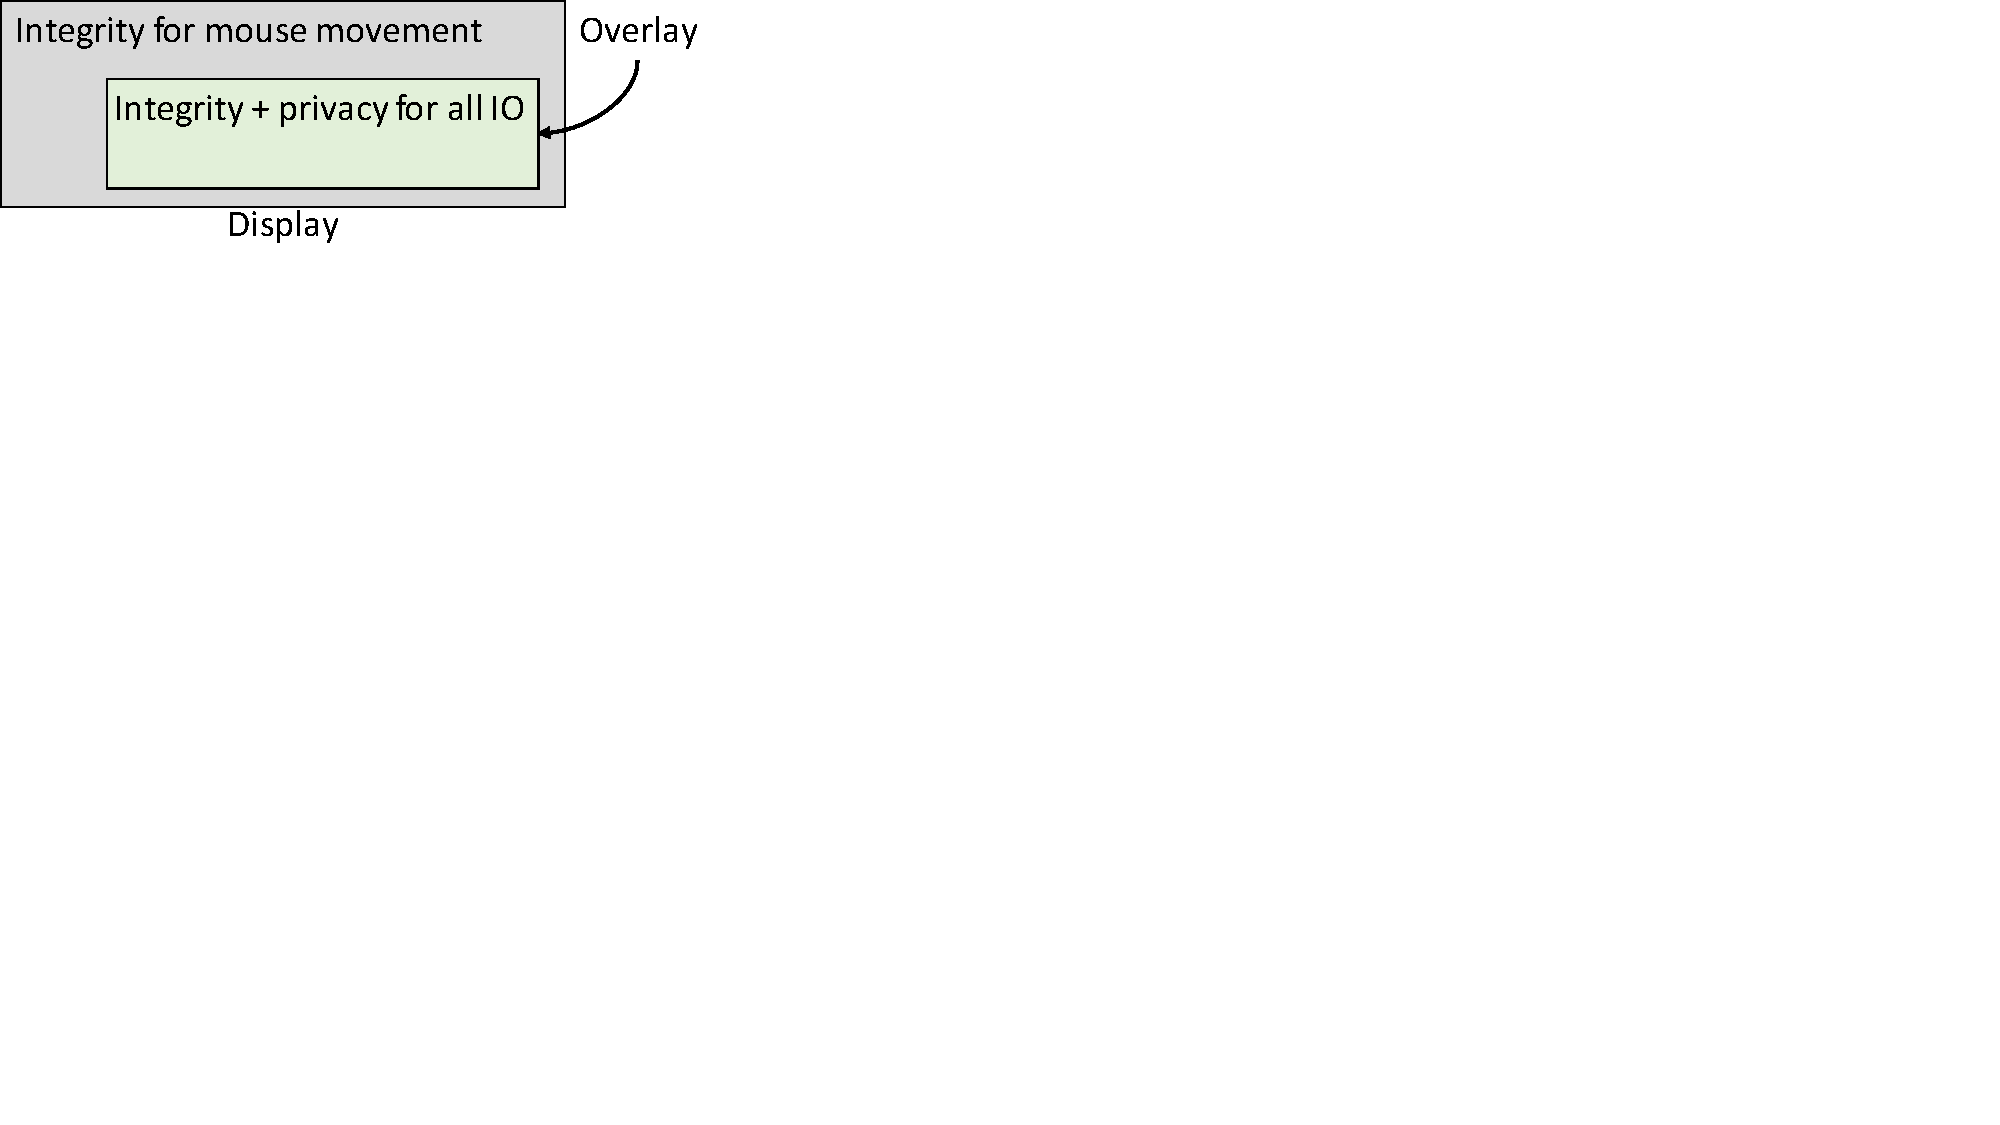
\includegraphics[trim={0 13cm 21.7cm 0}, clip, width=0.65\linewidth]{screenPartition.pdf}
\caption{\textbf{\device's pointer tracking, pointer \& UI overlay, and security properties.} Our proposed method provides two layers of protection for IO to the user. 1. In all the parts of the screen, the \device provide pointer integrity (the gray part). 2. The green part of the screen where the \device overlays on the HDMI stream where the \device provide integrity and privacy (privacy is dependent on the application requirements) for the IO.}
\label{fig:screenPartition}
\centering
\end{figure}
\fi

\begin{figure}[t]
\centering
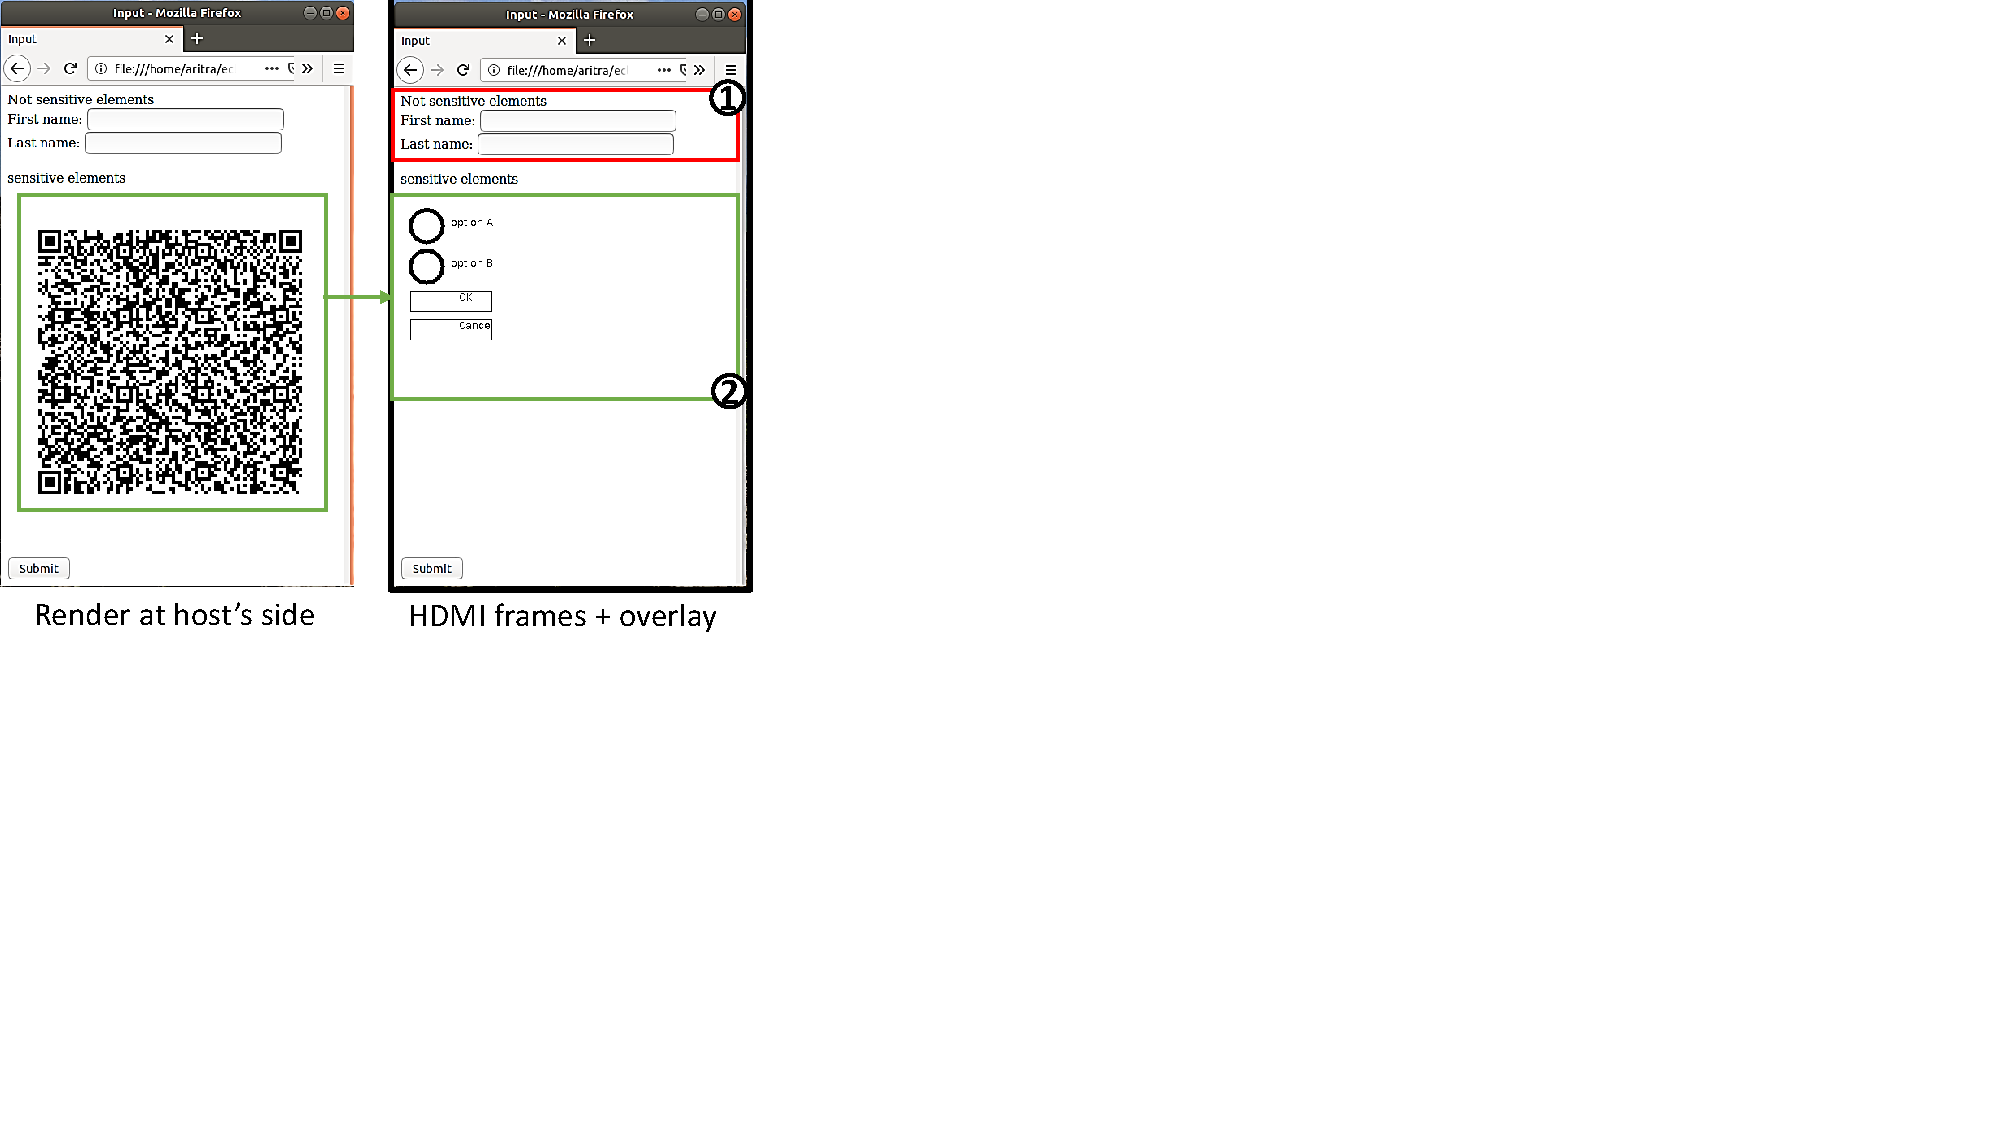
\includegraphics[trim={0 11cm 20cm 0}, clip, width=0.8\linewidth]{overlayScreenShot.pdf}
\caption{\textbf{\device generated UI overlay} that our solution use to hide the sensitive UI elements and inputs from the attacker-controlled host. Any input in the UI overlay is signed by the \device, hence the integrity of the user input is preserved.}
\label{fig:screenshot_1}
\centering
\end{figure}

\subsection{High-level Description of the System}

\name assumes that IO devices (mouse, keyboard, and display) are connected to a trusted component called \device. This setup allows the trusted \device to receive raw inputs from the user and show overlays on the display. The goal of \name is to keep the code running on the \device minimal and in the same time support a wide variety of applications. Thus, we avoid running any application, such as browsers, on the trusted component in order to keep the TCB very small.

The \device operates in two modes: passive and active. In the passive mode, the \device serves as a relaying device that forwards mouse and keyboard inputs to the host. Similarly, the \device relays the HDMI frames from the host to the display. Hence, the user experience is not affected when interacting with regular applications. On the active mode, \device has two functionalities: i) intercepts the inputs generated by the user, and ii) render overlays on the HDMI frame that is displayed on the screen. The first functionality guarantees that the user inputs arrive directly to a trusted component (\device), therefore, the compromised host cannot manipulate them. The second functionality allows the \device to show trusted information on the screen such as user inputs, or data sent from the remote server.

At the initialization phase, the \device and the remote server share a key that is used to encrypt/sign the communication between each-other. The remote server signs the sensitive elements that should be protected and delivers them to the untrusted host. The application running on the host encodes, e.g., using QR-codes, the sensitive elements into the HDMI frame. The \device captures the frames, decodes the sensitive elements, verifies their signatures, and then renders elements into an overlay. In this way, the device guarantees that the user is presented with the legitimate elements sent by the remote server and the user interaction with these elements is managed only by the device itself. User inputs (mouse events and keystrokes) addressed to the secured elements are intercepted by the \device and not forwarded to the untrusted host. Furthermore, the \device renders the user inputs into the overlay displayed on the screen, so the user experience is very similar to interacting with regular elements. 

\subsection{Challenges}

%Modern user interfaces are extremely complex to analyze, and such allows many possible ways to provide input. This makes the protection of IO integrity, and privacy is a particularly challenging task. For example, given a command from the user, it is necessary to understand the user intention that corresponds to the mouse movements. Given the screen space, there exist a multitude of ways for the user to move a mouse a place on a specific UI element that fires a command to the remote end system. To provide an end-to-end protection to this entire activity one needs to 1) precisely track the cursor position, 2) correspond the cursor location to the given movement data from the mouse, 3) understand the semantics of the UI element the fires the command, and 4) generate an efficient and comprehensive proof that the server can use to understand the user's real intention.

Modern user interfaces (UIs) are diverse and hard to generalize, resulting in many possible ways to provide input and receiving output.  This makes the protection of IO integrity, and privacy is a particularly challenging task. For example, given a mouse movement and clicking on a button from the user, it is necessary to understand the user intention that corresponds to the mouse movements. One naive solution would be to record a continuous screen capture of display and send it to the server. As the screen capture captures all the information displayed on the screen, later review should uncover if the attacker attempts to manipulate the UI or the IO data. Even though this naive solution provides strong security guarantee, it is impractical. So, the first challenge arises to build a secure system that is feasible and can be generalized with all the IO devices.   

The second challenge arises while ensuring IO confidentiality. For mouse input, hiding the mouse movement while keeping all the regular functionality intact is a challenging task as we do not consider large TCB-based solution such as a trusted hypervisor.`


Apart from these functional challenges for implementation, there exist multiple attack vectors that we want to provide protection. An attacker that controls the entire host can lunch complex UI-based attacks. Such includes spawning multiple mouse pointer to trick the user into following the wrong mouse pointer, changing the layout of the UI elements to trick the user into providing sensitive data, tricking the user into moving the mouse to the wrong location and click there, manipulate input data, etc.





\iffalse
\subsection{Approach}

The main objective of our approach is to provide a secure channel between the user IO devices and the remote server that provides integrity and privacy of the IO data. Our solution uses the \device as the IO \emph{root-of-trust}. The \device that can be either integrated into the graphics card or can be used as a stand-alone auxiliary device (as we did in our implementation). The \device taps into the HDMI channel extracts frames and determine the current context of the user's action. The \device also can overlay bitmaps into the HDMI channel. By doing this, the \device provides security properties to the IO devices that are illustrated in Figure~\ref{fig:screenPartition}. Using such capability, our system provides the following security properties: \emph{\pop}, \emph{\poui}, \emph{\poa}, and integrity and privacy of the IO.

\myparagraph{\Pop} All the keyboard and mouse input from the user is intercepted by the \device. The \device uses the raw mouse data from the user, and on the screen, it detects the corresponding position of the mouse pointer. The \device captures a trace of the mouse pointer position and the click data. Using the mouse trace data, the \device computes a \emph{\pop}. The \pop serves as an indirect measure for the input integrity as the \device confirms the remote server that if the user drags/clicks the mouse in a way that results in an input to the remote server. The \device also overlays a mouse-pointer image on the host's cursor. The overlaid mouse pointer is conspicuous to the user and uses as a safeguard if the host generates multiple pointers. Additionally, the \device employs secure attention sequence (SAS) mechanism that dims all of the display except the overlaid UI and the mouse pointer for user attention.

\myparagraph{\poa} \Poa guarantees that a specific command that is sent to the server is indeed issued legitimately by the user. Any action on the overlaid region of the screen is recorded and signed by the \device.  Direct inputs such as clicking a button or a text data in a text box are signed by the \device and sent to the remote server. These signed input data serves as the second-factor fort the input integrity. The server receives and matches the \emph{applications-level} payload from the browser and the \emph{signed second factor} from the \device. 

\myparagraph{\Poui} All the UI elements that are displayed on the overlaid area is rendered by the \device and signed by the remote server. \Poui ensures that a UI that is seen by the user is legitimately generated by the remote server and reconstructed faithfully by the \device. The JavaScript snippet that is served by the remote server transforms the security-critical UI of the webpage to a QR-code encoded specification. The \device detects the QR code by intercepting the HDMI frame between the host and the display \device. The specification is signed that provides the integrity and the authenticity of both the output data and the UI objects on the webpage. 

\myparagraph{IO integrity and privacy} As the \device also sits on the HDMI channel between the host and display \device, it can overlay objects on the HDMI stream and thus achieves display integrity and privacy. All the objects that are overlaid by the \device can only be seen by the user, and the host is oblivious to the IO.


\fi